\subsection{Baza danych}
Baza danych to zbiór danych istniejący przez długi czas który opisuję wybraną 
cześć świta rzeczywistego, w spójny logiczny sposób, zaprojektowany w konkretnym celu,
do którego dostęp ma konkretna grupa użytkowników. 
\subsubsection{Diagram związków encji}
Diagram związków encji (entity-relationship -E/R) jest jednym z formalizmów 
wykorzystywanych do projektowania bazy danych. Przedstawia on najważniejsze
części danych oraz powiązania między nimi za pomocą kształtów geometrycznych. 



W naszym przypadku należy rozwinąć kilka pojęć aby poprawnie zrozumieć
poniżej przedstawiane schematy:
\begin{itemize}
    \item \textbf{Atrybut} - najprostsza właściwość, wyraża w typach prostych cechy encji 
    \item \textbf{Encja} - reprezentacja pojedyńczego obiektu rzeczywistego lub wymyślonego
    \item \textbf{Związek} - zalezności występujące między encjami
\end{itemize}


\begin{figure}[htbp]
    \centering
    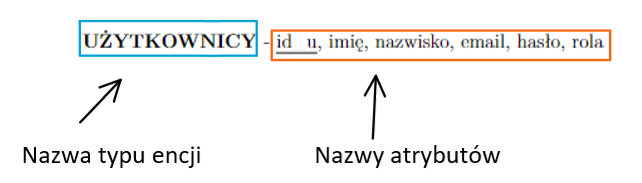
\includegraphics[width=0.7\textwidth]{Rozdziały/Opis zaprojektowanego systemu/Podrozdziały/LegendaODL.png}  % Ścieżka do pliku i szerokość obrazka
    \caption{Legenda Z}  % Podpis pod obrazkiem
    \label{fig:nazwa_etkiety}  % Etykieta do odwołań
\end{figure}




W przypadku naszego projektu bazy danych wyróżnić możemy następujące typy encji:
\begin{itemize}
    \item \textbf{UŻYTKOWNICY} - \underline{id\textunderscore{}u}, imię, nazwisko, email, hasło, rola
    \item \textbf{PRACE} - \underline{id\textunderscore{}p}, data, czas\textunderscore{}rozpoczęcia, czas\textunderscore{}zakończenia, przerwa\textunderscore{}początek, przerwa\textunderscore{}koniec, status
    \item \textbf{DYSPOZYCYJNOŚCI} - \underline{id\textunderscore{}d}, data, typ, godzina\textunderscore{}rozpoczęcia, godzina\textunderscore{}zakończenia, status
    \item \textbf{GRAFIKI\textunderscore{}DZIENNE} - \underline{id\textunderscore{}gd}, data, godziny\textunderscore{}do\textunderscore{}wyrobienia, status
    \item \textbf{ZESPOŁY} - \underline{id\textunderscore{}z}, nazwa, menedżer\textunderscore{}id
\end{itemize}

\begin{figure}[htbp]
    \centering
    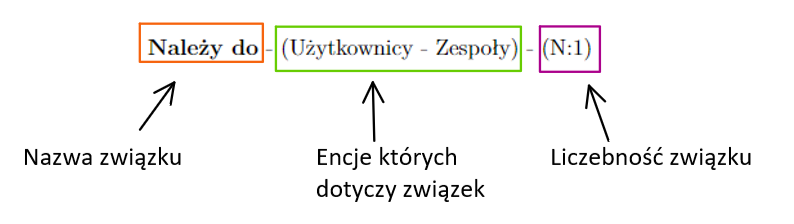
\includegraphics[width=0.7\textwidth]{Rozdziały/Opis zaprojektowanego systemu/Podrozdziały/LegendaZwiązki.png}  % Ścieżka do pliku i szerokość obrazka
    \caption{Legenda Z}  % Podpis pod obrazkiem
    \label{fig:nazwa_etkiety}  % Etykieta do odwołań
\end{figure}

Związki które reprezentują zależności występujące między encjami znajdują się poniżej:



\begin{itemize}
    \item  \textbf{Wykonał} - (Użytkownicy - Prace) - (1:N) 
    \item  \textbf{Podał} - (Użytkownicy - Dyspozycyjności) - (1:N)  
    \item \textbf{Należy do} - (Użytkownicy - Zespoły) - (N:1) 
    \item  \textbf{Dostał zmiane} - (Użytkownicy - Grafiki\textunderscore{}dzienne) - (N:M): godzina\textunderscore{}rozpoczęcia, godzina\textunderscore{}zakończenia
\end{itemize}

Powyższe dane zostały zebrane i przekształcone w graficzną reprezntacje diagramu związków encji
gdzie kształty kolejno oznaczają:
\begin{itemize}
 \item Romb - związek między encjami
 \item Prostokąt - Typ encji
 \item Strzałka - związek o liczebności jeden do wielu (N:1) - encja typu A może być związana z jedną encją typu B, zaś encja typu B może być związana z wieloma encjami typu A
 \item Linia - związek o liczebności wiele do wielu (N:M) - encja typu A może być związana z wieloma encjami typu B, jak i encja typu B może być związana z wieloma encjami typu A - taki związek w bazie ma swoje odzwierciedlenie jako niezależna tabela
\end{itemize}

\begin{figure}[htbp]
    \centering
    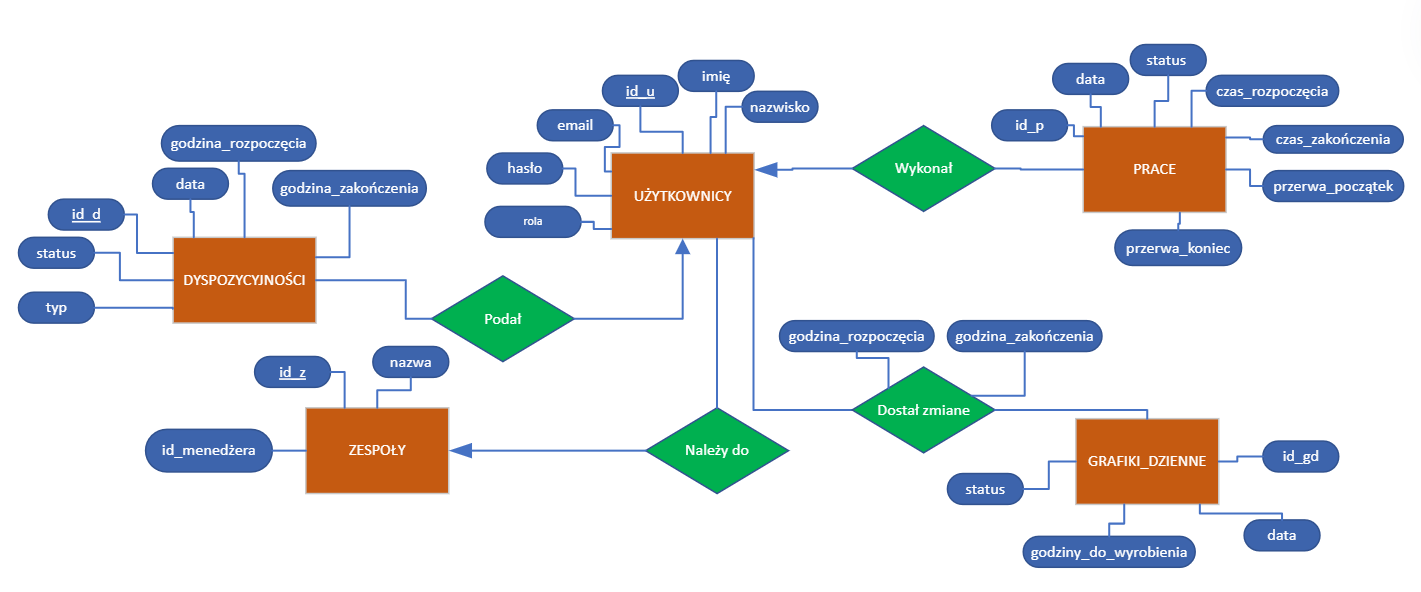
\includegraphics[width=1\textwidth]{Rozdziały/Opis zaprojektowanego systemu/Podrozdziały/DataBase.png}  % Ścieżka do pliku i szerokość obrazka
    \caption{Diagram związków encji}  % Podpis pod obrazkiem
    \label{fig:nazwa_etkiety}  % Etykieta do odwołań
\end{figure}


\subsubsection{Relacyjny model bazy danych}

Co to relacyjny model bazy danych?
Opisać tą tabelke 

\begin{figure}[htbp]
    \centering
    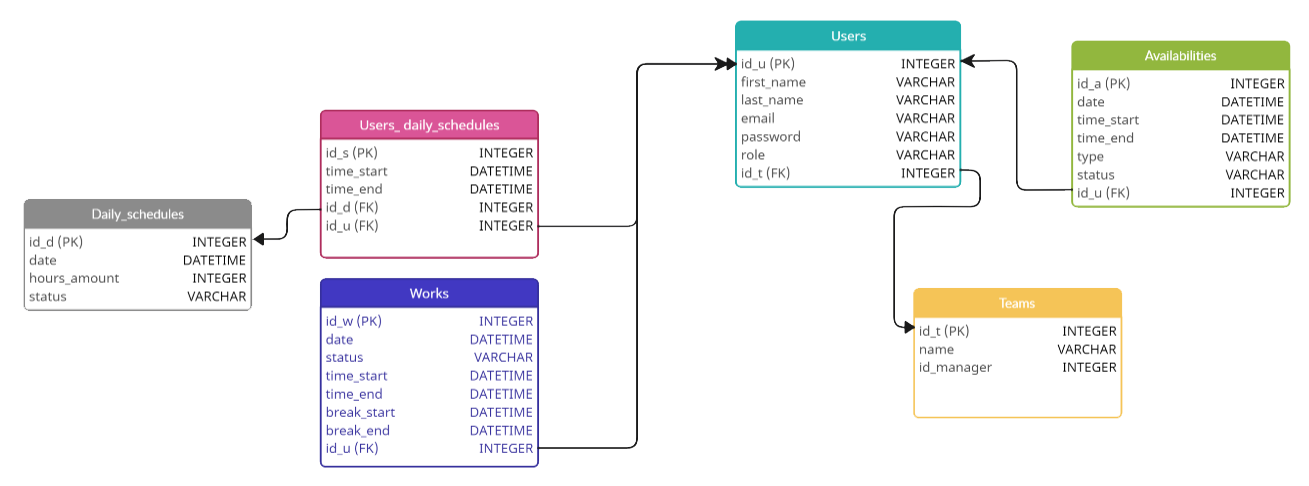
\includegraphics[width=1\textwidth]{Rozdziały/Opis zaprojektowanego systemu/Podrozdziały/DataBaseEN.png}  % Ścieżka do pliku i szerokość obrazka
    \caption{Relacyjny model bazy danych}  % Podpis pod obrazkiem
    \label{fig:nazwa_etkiety}  % Etykieta do odwołań
\end{figure}

Opis tabel znajdujących się w bazie

\begin{table}[h!]
    \centering
    \begin{tabular}{|p{3cm}|p{6cm}|p{4cm}|}
    \hline
    \textbf{Kolumna} & \textbf{Opis} & \textbf{Typ danych} \\ \hline
    id\_u & Uniklany identyfikator użytkownika & PK, AI, INTEGER\\ \hline
    email &   Email użytkownika & VARCHAR \\ \hline
    first\_name &   Imie użytkownika & VARCHAR \\ \hline
    last\_name &   Nazwisko użytkowika & VARCHAR \\ \hline
    password & Hasło użytkownika  & VARCHAR \\ \hline
    role & Rola użytkownika & VARCHAR \\ \hline
    id\_t & Klucz obcy wskazujący na krotke z tabeli TEAMS   & FK, INTEGER \\ \hline
    \end{tabular}
    \caption{Tabela - Users (odpowiada encji UŻYTKOWNICY)}
\end{table}

\begin{table}[h!]
    \centering
    \begin{tabular}{|p{3cm}|p{6cm}|p{4cm}|}
    \hline
    \textbf{Kolumna} & \textbf{Opis} &\textbf{Typ danych}  \\ \hline
    id\_t & Unikalny identyfikator zespołu &  PK, AI, INTEGER\\ \hline
    name & Nazwa zespołu & VARCHAR\\ \hline
    id\_manager & Idetyfikator menedżera & INTEGER \\ \hline
    \end{tabular}
    \caption{Tabela - Teams (odpowiada encji ZESPOŁY)}
\end{table}

\begin{table}[h!]
    \centering
    \begin{tabular}{|p{3cm}|p{6cm}|p{4cm}|}
    \hline
    \textbf{Kolumna} & \textbf{Opis} & \textbf{Typ danych} \\ \hline
    id\_a & Unikalny identyfikator dostępności pracownika & PK, AI, INTEGER \\ \hline
    time\_start & Godzina od której zaczyna się dostępność pracownika w danym dniu &  DATETIME\\ \hline
    time\_end & Godzina do której kończy się dostępność pracownika w danym dniu & DATETIME \\ \hline
    date & Data określająca dzień na który podawana jest dostępność  & DATETIME \\ \hline
    status & Status określający czy nadal istenieje możlwiość edytcji podanej dostępnosci & VARCHAR\\ \hline
    type & Typ określający czy dostępność podawana przez pracownika jest między określanymi godzinami czy całodniowa & VARCHAR \\ \hline
    id\_u & Klucz obcy wskazujący na krotke z tabeli Users & FK, INTEGER \\ \hline
    \end{tabular}
    \caption{Tabela - Availability (odpowiada encji DOSTEPNOŚCI)}
\end{table}

\begin{table}[h!]
    \centering
    \begin{tabular}{|p{3cm}|p{6cm}|p{4cm}|}
    \hline
    \textbf{Kolumna} & \textbf{Opis} & \textbf{Typ danych} \\ \hline
    id\_w & Uniklany identyfikator rejestru godzin przepracowanych przez pracownika &PK, AI, INTEGER \\ \hline
    date & Data określająca dzień pracy pracownika & DATETIME\\ \hline
    status & Status określający czy można edytować przepracowane godziny pracownika & VARCHAR\\ \hline
    time\_start & Godzina od której nalicza się czas pracy pracownika & DATETIME\\ \hline
    time\_end & Godzina do której nalicza się czas pracy pracownika & DATETIME \\ \hline
    break\_start & Godzina od której nalicza się czas przerwy pracownika & DATETIME \\ \hline
    break\_end &  Godzina do której nalicza się czas przerwy pracownika & DATETIME\\ \hline
    id\_u & Klucz obcy wskazujący na krotke z tabeli Users & FK, INTEGER \\ \hline
    \end{tabular}
    \caption{Tabela - Work (odpowiada encji Prace)}
\end{table}

\begin{table}[h!]
    \centering
    \begin{tabular}{|p{3cm}|p{6cm}|p{4cm}|}
    \hline
    \textbf{Kolumna} & \textbf{Opis} & \textbf{Typ danych} \\ \hline
    id\_d & Uniklany identyfikator grafiku na konkretny dzień & PK, AI, INTEGER \\ \hline
    date & Data grafiku & \\ \hline
    hours\_amount & Określona lość godzin do obłożenia przez pracowników  &  INTEGER\\ \hline
    status & Status określający czy grafik jest gotowy do publikacji & VARCHAR \\ \hline
    \end{tabular}
    \caption{Tabela - Daily\_Schedule (odpowiada encji GRAFIKI\_DZIENNE)}
\end{table}

\begin{table}[h!]
    \centering
    \begin{tabular}{|p{3cm}|p{6cm}|p{4cm}|}
    \hline
    \textbf{Kolumna} & \textbf{Opis} & \textbf{Typ danych} \\ \hline
    id\_s & Uniklany identyfikator grafiku na konkretny dzień dla konkretnego pracownika & PK, AI, INTEGER \\ \hline
    time\_start & Godzina określająca planowy czas rozpoczęcia pracy przez pracownika & DATETIME \\ \hline
    time\_end & Godzina określająca planowy czas zakończenia pracy przez pracownika & DATETIME\\ \hline
    id\_d & Klucz obcy wskazujący na krotke z tabeli Daily\_Schedule & FK, INTEGER\\ \hline
    id\_u & Klucz obcy wskazujący na krotke z tabeli Users & FK, INTEGER\\ \hline
    \end{tabular}
    \caption{Tabela - UserDaily\_Schedule (odpowiada związkowi wieloargumentowemu Dostał zmiane)}
\end{table}
